\documentclass[xcolor=table]{beamer}

\usepackage{lscape, amsmath, amsfonts, amssymb, setspace, theorem, wrapfig, graphicx, float, multirow, subfig, color, rotating, multicol, datetime, natbib, venndiagram, pstricks, xkeyval, tikz, etoolbox, verbatim, subfig}

\usepackage{listings}
\usepackage{xcolor}
 
\definecolor{codegreen}{rgb}{0,0.6,0}
\definecolor{codegreengray}{rgb}{0,0.4,0}
\definecolor{codegray}{rgb}{0.5,0.5,0.5}
\definecolor{codeblue}{rgb}{0.00,0,0.82}
\definecolor{backcolour}{rgb}{0.95,0.95,0.92}
 
\lstdefinestyle{mystyle}{
    backgroundcolor=\color{backcolour},   
    commentstyle=\color{codegreengray},
    numberstyle=\tiny\color{codegray},
    stringstyle=\color{codegreen},
    basicstyle=\ttfamily\footnotesize,
    breakatwhitespace=false,         
    breaklines=true,                 
    captionpos=b,                    
    keepspaces=true,                 
    numbers=left,                    
    numbersep=5pt,                  
    showspaces=false,                
    showstringspaces=false,
    showtabs=false,                  
    tabsize=2
}
 
\lstset{style=mystyle}

\title{GV300 - Quantitative Political Analysis}
\subtitle{University of Essex - Department of Government}
\date{Week 9 -- 25 November, 2019}				% or you can specify a date, just write it down instead of "\today"
\author{Lorenzo Crippa} 

\usetheme[progressbar=frametitle]{metropolis}
\usecolortheme{seahorse}						% try others: wolverine; crane...


\begin{document}
\frame{
\titlepage
}

\frame{
\frametitle{Problem Set 3.1}
\begin{enumerate}
\item (10 marks) Expectation of random variables:
	\begin{enumerate}
	\item[(a)] (5 marks) Show for arbitrary random variable $X$ that $V(X)=E[X^2]-E[X]^2$. Think about how you could express the variance $V(X)$ in terms of expectation so that you end up with the term on the right hand side of the equation (Hint: look at the slides covering random variables and expectation). Arbitrary means, you could plug in any random variable and should get the equation to hold.\\
	\item[(b)] (5 marks) Is it \textbf{generally} true that $E[f(x)]$ = $f(E[x])$ for arbitrary random variable $f$? Show your reasoning.
	\end{enumerate}
\end{enumerate}
}

\frame{
\frametitle{Problem Set 3.1}
\begin{enumerate}
\item[(a)] \begin{itemize}
	\item[] $V(X) = E[(X - \mu)^2] = E[X^2 - 2\mu X + \mu^2]$
    \item[]     $= E[X^2] - E[2\mu X] + E[\mu^2] = E[X^2] - 2\mu E[X] + \mu^2$
    \item[]     $= E[X^2] - 2\mu (\mu) + \mu^2= E[X^2] - 2\mu^2 + \mu^2$
    \item[]     $= E[X^2] - \mu^2 = E[X^2] - E[X]^2$
\end{itemize} \pause

\item[(b)] ``Generally''. You only need to find one example to disprove the proposition! Take $f(x)=x^2$ as example. Say $X=\{1,2,3,4\}$ with associated probabilities $.25,.25,.25,.25$, respectively. $X^2$ is then $\{1,4,6,8\}$ and so $E[X]=.25*1 + .25*4 + .25*9 + .25*16 = 7.5$ but $E[X]^2=(.25*1 + .25*2 + .25*3 + .25*4)^2 = 2.5^2 = 6.25$. %Note,  (1.b) is linked to (1.a) in that you showed in (a) what the variance of X is (and it is not 0!). This example here in (b) is nothing else than an example for (1.a) so the equation in (1.b) cannot hold otherwise (1.a) could not have been true.
\end{enumerate}
}

\frame{
\frametitle{Problem Set 3.2}
\begin{enumerate}
\item[2.] (7 marks) Simulate, that is randomly draw, 5000 observations of a variable following a binomial distribution with success probability $.3$ and $12$ trials. 
	\begin{enumerate}
	\item[(a)] (3 marks) Write down a verbal definition of probability mass function (PMF), probability density function (PDF), and cumulative distribution function (CDF); check any text book if necessary for CDF, we covered PMF (for categorical random variables) and PDF (for continous random variables) already.\\

	\item[(b)] (4 marks) Plot PMF and CDF of the variable you created.
	\end{enumerate}
\end{enumerate}
}

\frame{
\frametitle{Problem Set 3.2 (a)}
\begin{enumerate}
\item[(a)] A listing of the values taken by a random variable and their associated probabilities is a probability distribution. The probabilities associated with each individual value of a discrete random variable is called probability mass function. For the continuous case, the probability associated with any particular point is zero but the probabilities associated with intervals in the range of values of the variable are defined by the probability density function. The cumulative distribution function gives the probability that the values of a random variable are less than or equal to a specific value
\end{enumerate}
}

\begin{frame}[fragile]
\frametitle{Problem Set 3.2 (b) -- R}
Solution in R:
\begin{lstlisting}[language = R]
set.seed(1111)
x <- rbinom(5000, p = .3, size = 12)

# PMF:
barplot(height = table(factor(x))/length(x),
        ylab = "frequency",
        xlab = "values",
        main = "PMF of x",
        ylim = c(0, 0.25))
        
# CDF:
barplot(height = cumsum(table(factor(x)))/length(x),
        ylab = "cumulative frequency",
        xlab = "values",
        main = "CDF of x",
        ylim = c(0, 1))
\end{lstlisting}
\end{frame}

\frame{
\frametitle{Problem Set 3.2 (b) -- R outputs}
\begin{figure}
  \centering
  \subfloat{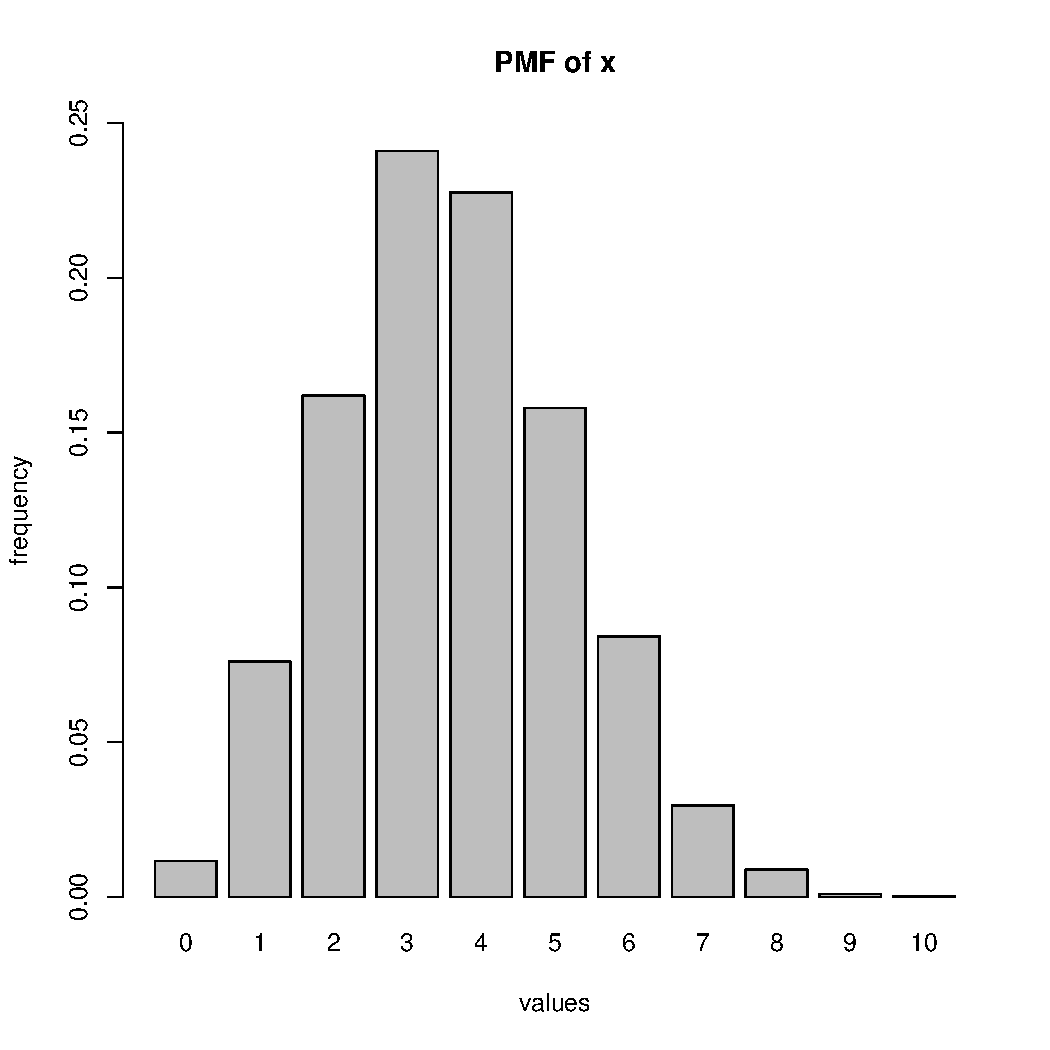
\includegraphics[width=50mm]{pictures/PMF.pdf}}\qquad
  \subfloat{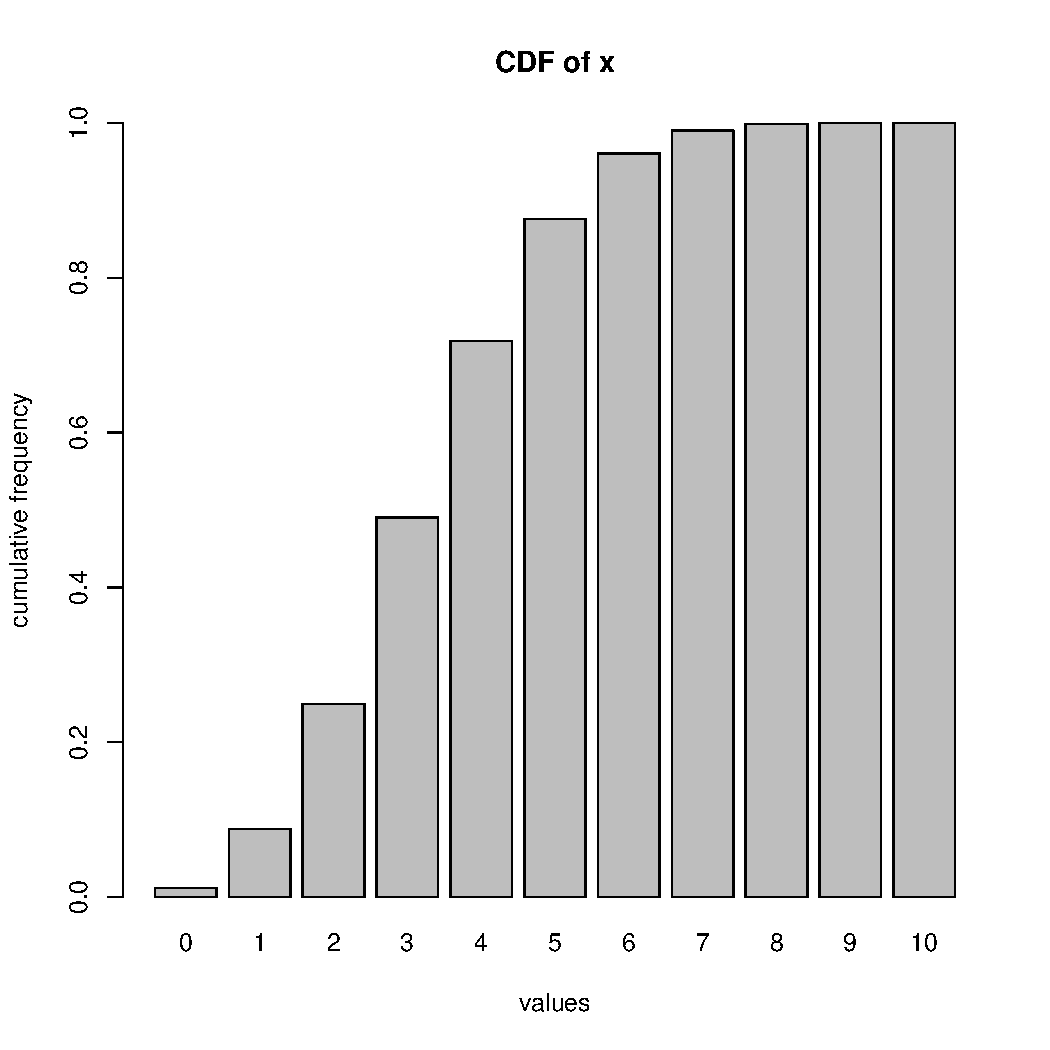
\includegraphics[width=50mm]{pictures/CDF.pdf}}
\label{fig:fig}
\end{figure}
}

\begin{frame}[fragile]
\frametitle{Problem Set 3.2 (b) -- Stata}
Solution in Stata:
\begin{lstlisting}[language = R]
set obs 5000

set seed 1111
gen x = rbinomial(12, .3)

*PMF
histogram x, fraction ytitle("frequency")

*CDF
cumul x, generate(y) equal
sort y

scatter y x, ytitle("cumulative frequency")

\end{lstlisting}
\end{frame}

\frame{
\frametitle{Problem Set 3.2 (b) -- Stata outputs}
\begin{figure}
  \centering
  \subfloat{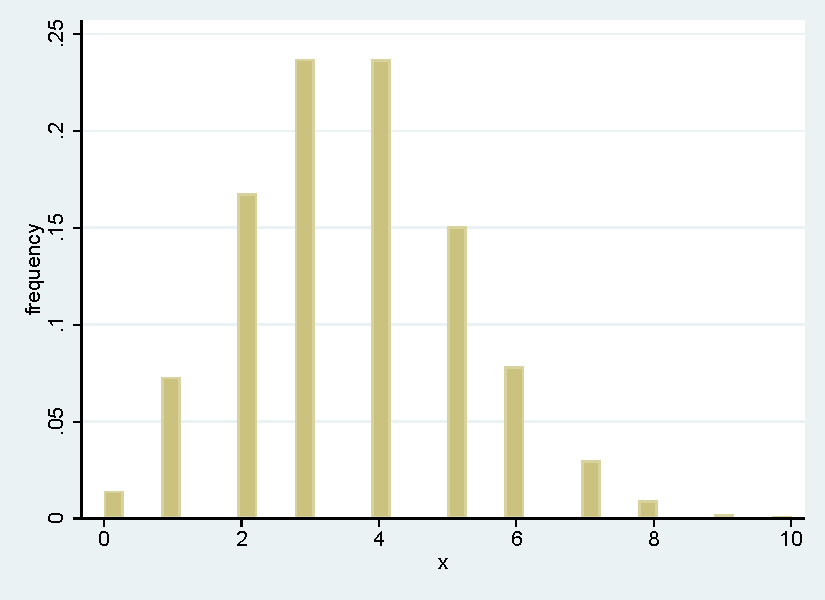
\includegraphics[width=50mm]{pictures/PMF_stata.pdf}}\qquad
  \subfloat{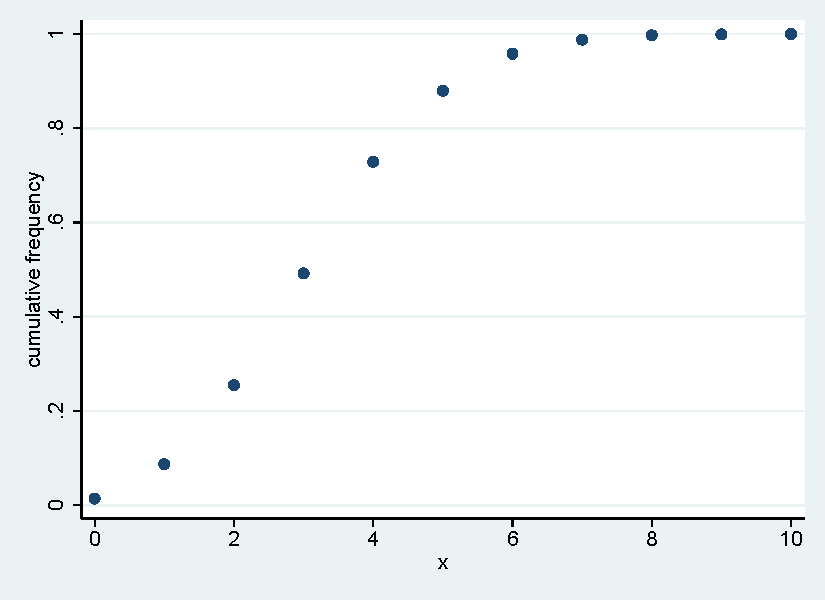
\includegraphics[width=50mm]{pictures/CDF_stata.pdf}}
\label{fig:fig}
\end{figure}
}

\frame{
\frametitle{Problem Set 3.3}
\begin{enumerate}
\item[3.] (16 marks) Variable $X^*$ is the standardized random variable for random variable $X$. 
It is given by $x^* = \frac{x-E[x]}{\sigma_x}$. 
This exercise asks you to plug in the terms given to you into the formula for expectation, variance, and correlation. Then simplify until you end up with a numeric solution (there is one).
	\begin{enumerate}
	\item[(a)] (8 marks) Compute expected value and variance for $x^*$ and show your steps of the computation?
	\item[(b)] (8 marks) Another statistic of interest, the correlation coefficient $\rho$ for random variables $X$ and $Y$ is defined to be
\[\rho_{XY}=E[x^*y^*]\]
Consider the definition of $x^*$ (also apply to $y^*$) and determine the numerical value of $\rho_{XY}$ if
		\begin{itemize}
		\item[(i)] $x=ay$ where $a>0$]
		\item[(ii)] $X$ and $Y$ are independent
		\end{itemize}
	\end{enumerate}
\end{enumerate}
}

\frame{
\frametitle{Problem Set 3.3 (a)}
$E[x^*]=E[\frac{x-E[x]}{\sigma_x}]=\frac{1}{\sigma_x}(E[x]-E[E[x]])=0$\\
$V[x^*]=E[x^{*^2}]-E[x^*]^2$ which you have shown in problem 1, also note you just got $E[x^*]=0$ so $E[x^*]^2=0$\\
That means $V[x^*]=E[x^{*^2}]-E[x^*]^2=E[(\frac{x-E[x]}{\sigma_x})^2]$\\
Then, rewrite $E[(\frac{x-E[x]}{\sigma_x})^2]=E[\frac{(x-E[x])^2}{\sigma_x^2}]=\frac{1}{\sigma_x^2}E[(x-E[x])^2]$\\
Invoking what we started from in problem 1, remember that $V(x)=E[(x-E[x]^2)]$ so we end up with $V[x^*]=\frac{1}{\sigma_x^2}V(x)$\\
Finally, $V(x)=\sigma_x^2$ so we got  $V[x^*]=\frac{1}{\sigma_x^2}V(x)=\frac{1}{\sigma_x^2}\sigma_x^2=1$\smallskip

Summarising, $E[x^*]=0$ and $V[x^*]=1$ as it should be the case for a standardized random variable
}

\frame{
\frametitle{Problem Set 3.3 (b)}
\[\rho_{XY}=E[x^*y^*]\]
Consider the definition of $x^*$ (also apply to $y^*$) and determine the numerical value of $\rho_{XY}$ if
\begin{itemize}
\item[(i)] $x=ay$ where $a>0$
\item[] $\rho_{XY}=\frac{E[(x-E[x])(y-E[y])]}{\sigma_X\sigma_Y}=\frac{E[(ay-E[ay])(y-E[y])]}{\sigma_X\sigma_Y}$
\item[] The numerator becomes: $=aE[(y-E[y])^2]=aV[y]$ (again, problem 1). Then, $V[x]=V[ay]=a^2V[y]$ therefore $\sigma_X\sigma_Y=\sqrt{a^2V[y]}\sqrt{V[y]}=aV[y]$ since $a>0$
\item[] Then, $\rho_{XY}=\frac{aV[y]}{aV[y]}=1$
\item[(ii)] $X$ and $Y$ are independent
\item[] Given independence, $E[XY]=E[X]E[Y]$, since we already computed $E[x^*]=0$, $\rho_{XY}=0$   
\end{itemize}
}

\frame{
\frametitle{Problem Set 3.4}
\begin{enumerate}
\item[4.] (22 marks) Consider the following table showing random variable $X$ which captures the number of terror attacks recorded in a sample of large cities with a population larger than 1 Million ($X_l$) and a sample of smaller cities with a population below 100000 ($X_s$). 
\begin{table}[H]\centering
\begin{tabular}{l|cccccccccc|r}\hline
	  &    &   &   &  	&   &  	 &   &    &   &   & n\\\hline
$X_l$ & 11 & 4 & 2 & 10 & 8 & 13 & 8 & 12 &   &   & 8\\\hline
$X_s$ & 14 & 2 & 2 & 6  & 12 & 2 & 4 & 1  & 1 & 7 & 10\\\hline
\end{tabular}	
\end{table}
We are interested in whether larger cities are more threatened by terror attacks
\end{enumerate}
}

\begin{frame}[fragile]
\frametitle{Problem Set 3.4 (a)}
\begin{itemize}
\item[(a)] (5 marks) Provide meaningful summary statistics and plot(s) to present the data \pause
\end{itemize}
In R:
\begin{lstlisting}[language = R]
df <- data.frame(xs = c(11,4,2,10,8,13,8,12,NA,NA),
                 xl = c(14,2,2,6,12,2,4,1,1,7))

describe(df, na.rm = T)
boxplot(df$xs, frame = F, ylab = "xs", 
        main = "boxplot of xs")
boxplot(df$xl, frame = F, ylab = "xl", 
        main = "boxplot of xl")
\end{lstlisting}
\end{frame}


\begin{frame}[fragile]
\frametitle{Problem Set 3.4 (a)}
In Stata:
\begin{lstlisting}
set obs 10

gen xl = .
replace xl = 11 if _n == 1
replace xl = 4 if _n == 2
...REPLACE MANUALLY...

gen xs = .
replace xs = 14 if _n == 1
replace xs = 2 if _n == 2 | _n == 3 | _n == 6
...REPLACE MANUALLY...

sum
graph box xl
graph box xs
\end{lstlisting}
\end{frame}

\begin{frame}
\frametitle{Problem Set 3.4 (a) -- R Outputs}
\begin{figure}
  \centering
  \subfloat{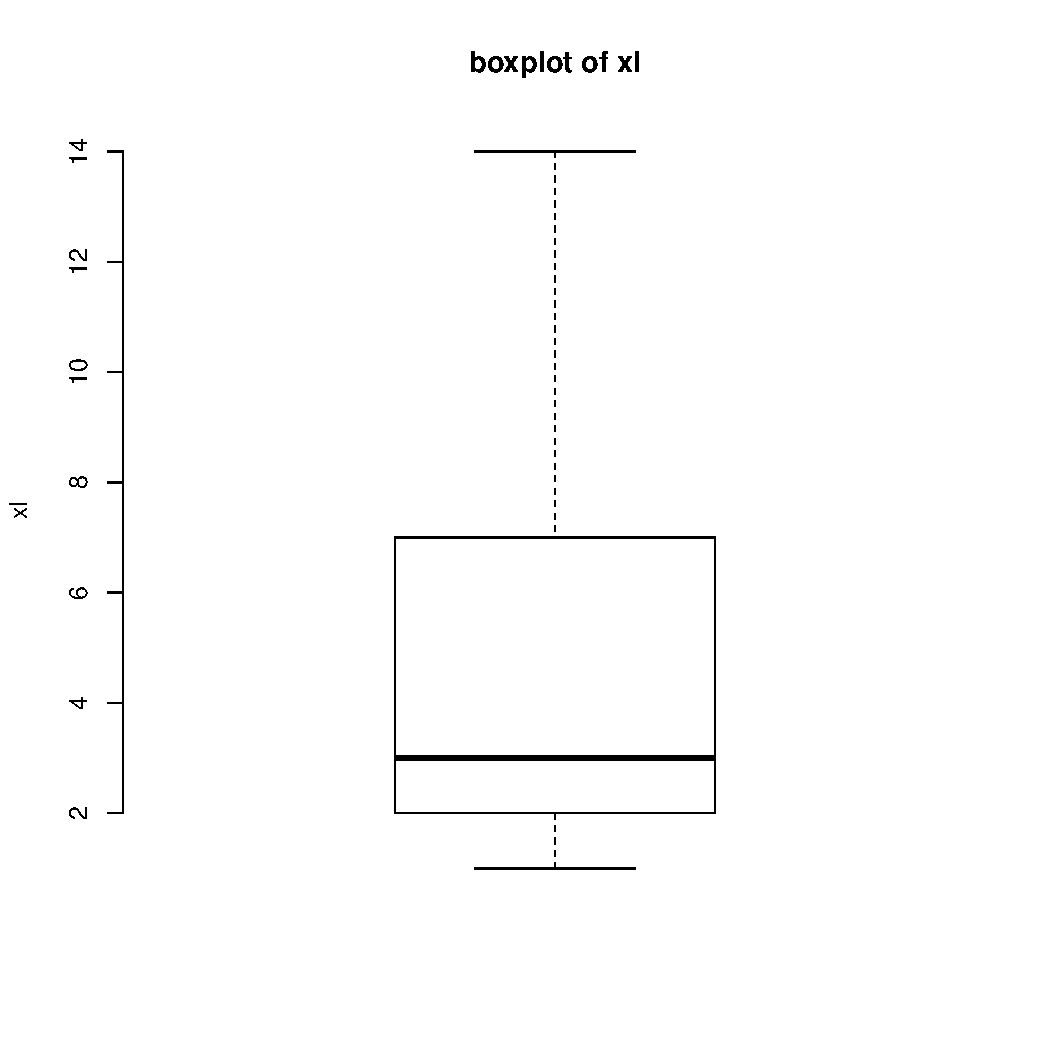
\includegraphics[width=50mm]{pictures/problem_set3_boxplot_xl.pdf}}\qquad
  \subfloat{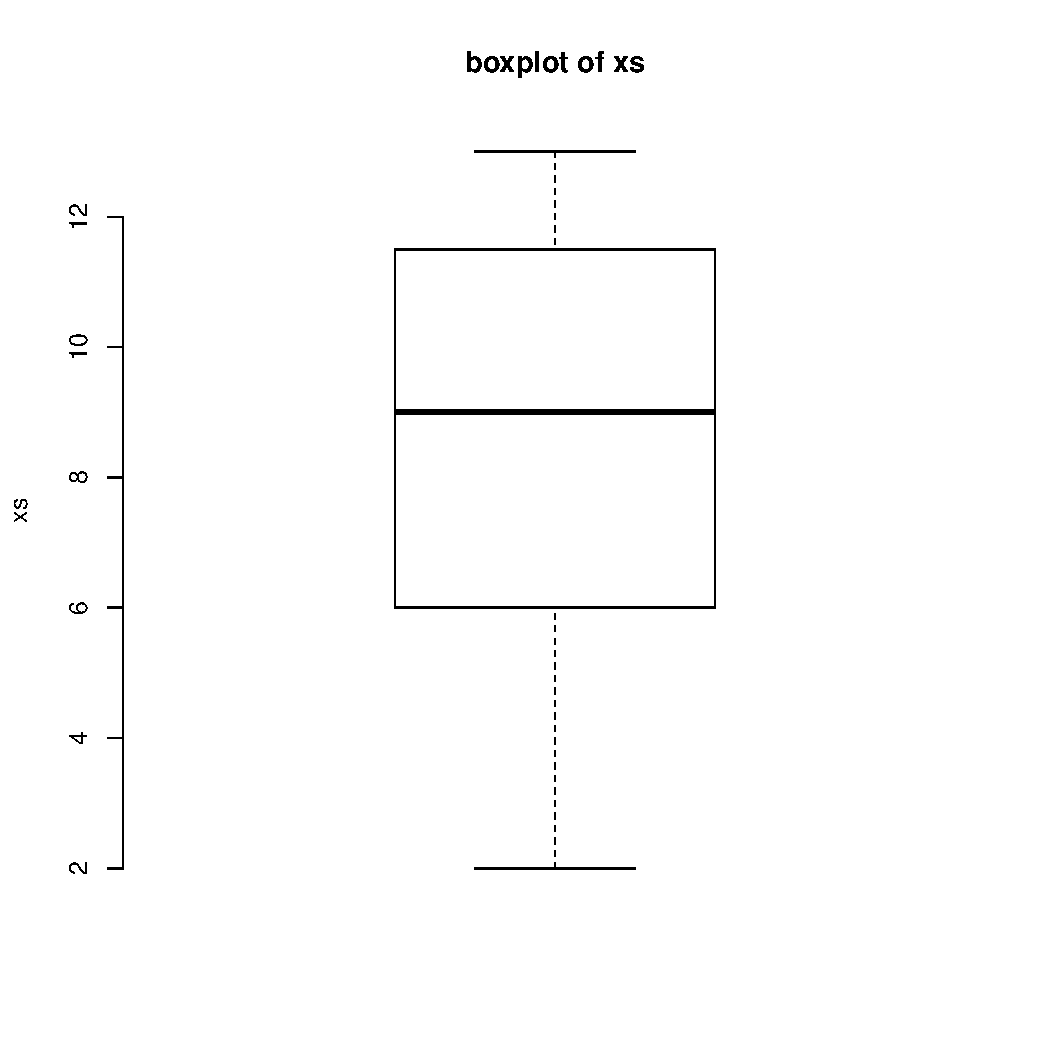
\includegraphics[width=50mm]{pictures/problem_set3_boxplot_xs.pdf}}
\label{fig:fig}
\end{figure}
\end{frame}

\frame{
\frametitle{Problem Set 3.4 (b)}
\begin{itemize}
\item[(b)] (2 marks) Write down a \textbf{null} hypothesis that speaks to our research interest. \pause \\
Null hypothesis: Larger cities do not experience more terror attacks than smaller cities.
\end{itemize}
}


\frame{
\frametitle{Problem Set 3.4 (c)}
\begin{itemize}
\item[(c)] (5 marks) The t-statistic for an equality in means test implemented by a t-test is
$$t^{sample} = \frac{|\overline{X}_l - \overline{X}_s |}{\sigma_{X_l,X_s}\sqrt{\frac{1}{n_l}+\frac{1}{n_s}}}$$ \\
And $\sigma_{X_l,X_s}^2 = \frac{(n_l-1)\sigma_{X_l}^2 + (n_s-1)\sigma_{X_s}^2}{(n_l+n_s-2)}$ \\
Compute $t^{sample}$ and show your calculations. 
The degrees of freedom here is given by $(n_l+n_s-2)$.\\ \pause
\[
t^{sample} = \frac{|8.5 - 5.1|}{\sqrt{\frac{(8-1)14.86 + (10-1)21.66}{8 + 10 - 2}} \sqrt{\frac{1}{8} + \frac{1}{10}}}  = 1.66
\]
\end{itemize}
}

\begin{frame}
\frametitle{Problem Set 3.4 (d)}
\begin{itemize}
\item[(d)] (5 marks) Consult your preferred statistical software and determine the probability of obtaining a t-statistic that is at least as large or larger than $t^{sample}$. Show how you got there by providing the Stata/R-code you wrote (if necessary consult heplfiles which Stata/R-command gives you the probability $P(T\geq t^{sample})$). Which quantity of interest did you just compute? How does it speak to the null hypothesis we formulated in (a)?\\ 
\end{itemize}
\end{frame}


\begin{frame}[fragile]
\frametitle{Problem Set 3.4 (d)}
\begin{itemize}
\item[(d)] $Pr(T\geq t^{sample}) = 1 - Pr(T<t^{sample})$. 
\\ From R:
\begin{lstlisting}[language = R]
> 1 - pt(tstat, df = 16)
[1] 0.05448782
\end{lstlisting}
\end{itemize}

This is the p-value associated with the test of the null hypothesis that large cities do not experience more terror attacks then small cities. \\
The probability of obtaining a t-statistic as large as the one we measure for random sampling reasons under the null hypothesis is $0.054$. \\
We can reject that null hypothesis with conventional level of significance of $0.1$. The mean number of terror attacks in large cities is significantly higher than in small cities. 
\end{frame}

\begin{frame}[fragile]
\frametitle{Problem Set 3.4 (e)}
\begin{itemize}
\item[(e)] (5 marks) Use your preferred statistical software, insert the data given in the table and run a t-test. Print the test result, interpret, and compare to your calculations by hand in (c) and (d). \\ \pause
In R:
\begin{lstlisting}[language=R]
t.test(x = df$xl, y = df$xs, alternative = "less", conf.level = .95)
\end{lstlisting} \pause

In Stata:
\begin{lstlisting}
ttest xs == xl
\end{lstlisting} \pause

\item[] Good point from Dominik: ``Check precise definition of test in R. Often the degree of freedom adjustments vary. The \texttt{t.test()} command in R adjusts the degrees of freedom by taking into account the variances in the two samples.''
\end{itemize}
\end{frame}

\frame{
\frametitle{Problem Set 3.5}
\begin{enumerate}
\item[5.] (12 marks) Find a poll conducted in the UK in 2019 that aims to measure citizens' preferences over environmental policies.
\begin{enumerate}
	\item[(a)] (8 marks) Obtain detailed information about the methodology of the survey, in particular, about the sampling of respondents. Describe the methodology in one paragraph referencing the distinction population and sample in depth.  
\end{enumerate}
\end{enumerate}
\pause
A discussion of the methodology should provide at least:
\begin{itemize}
	\item Definition of the population of interest
	\item Type of sample (i.e. representative, convenience, probability sample)
	\item Information on the survey mode (i.e. face-to-face, phone, online)
	\item Information on sampling strategy 
\end{itemize}
}

\frame{
\frametitle{Problem Set 3.5}
\begin{enumerate}
\item[(b)] (4 marks) Can you think of other reasons, other than resulting from the problems associated with sampling correctly from the population of interest, which may bias our measure of voter's preference in such a survey? Deliver at least two other reasons and discuss in 2-3 sentences.
\end{enumerate}
\pause
Issues that come to mind are:
\begin{itemize}
\item Respondents may not want to give a valid response 
\item Respondents may not be able to give a valid response
\item Sampling issues
\item Biases due to mode of survey or surveyor biases
\end{itemize}
}



\begin{frame}
\frametitle{Problem Set 3.6 (a)}
\begin{enumerate}
\item[6.] (18 marks) Program functions in R, program programs in Stata; remember to provide code and output in your solution:
\begin{enumerate}
\item[(a)] (5 marks) Generate 50 observations of 100 $\chi^2$ (that's ``chi square'') distributed variables with 50 degrees of freedom (that's the parameter to consider when specifying a draw from a $\chi^2$ distribution). 
Create a new variable, which is the average of each of these 100 $\chi^2$ distributed variables and create a histogram of this variable (this will be a sample of 100 observations). 
\end{enumerate}
\end{enumerate}
\end{frame}

\begin{frame}[fragile]
\frametitle{Problem Set 3.6 (a)}
In R:
\begin{lstlisting}[language = R]
mat <- matrix(rep(NA, 5000), nrow = 50, ncol = 100)
for (i in 1:100) {
  set.seed(i+142) # every iteration a different seed
  mat[,i] <- rchisq(n = 50, df = 50)
}

mean <- array(data = NA, dim = 100)
for (i in 1:100) {
  mean[i] <- mean(mat[,i])
}

hist(mean, col = "gray")
\end{lstlisting}
\end{frame}

\begin{frame}[fragile]
\frametitle{Problem Set 3.6 (a)}
In Stata:
\begin{lstlisting}
program drop _all
program define rchisq, rclass
	drop _all
	set obs 50
	tempvar mu
	g `mu' = rchi2(50)
	sum `mu'
	return scalar mu = r(mean)
end

simulate mu=r(mu), reps(100) saving(sim, replace): ///
	rchisq
	
use sim, clear
hist mu, col(gray) name(hist50, replace) ///
	ti("Histogram of mean", col(black))
\end{lstlisting}
\end{frame}

\frame{
\frametitle{Problem Set 3.6 (a) -- output}
\begin{center}
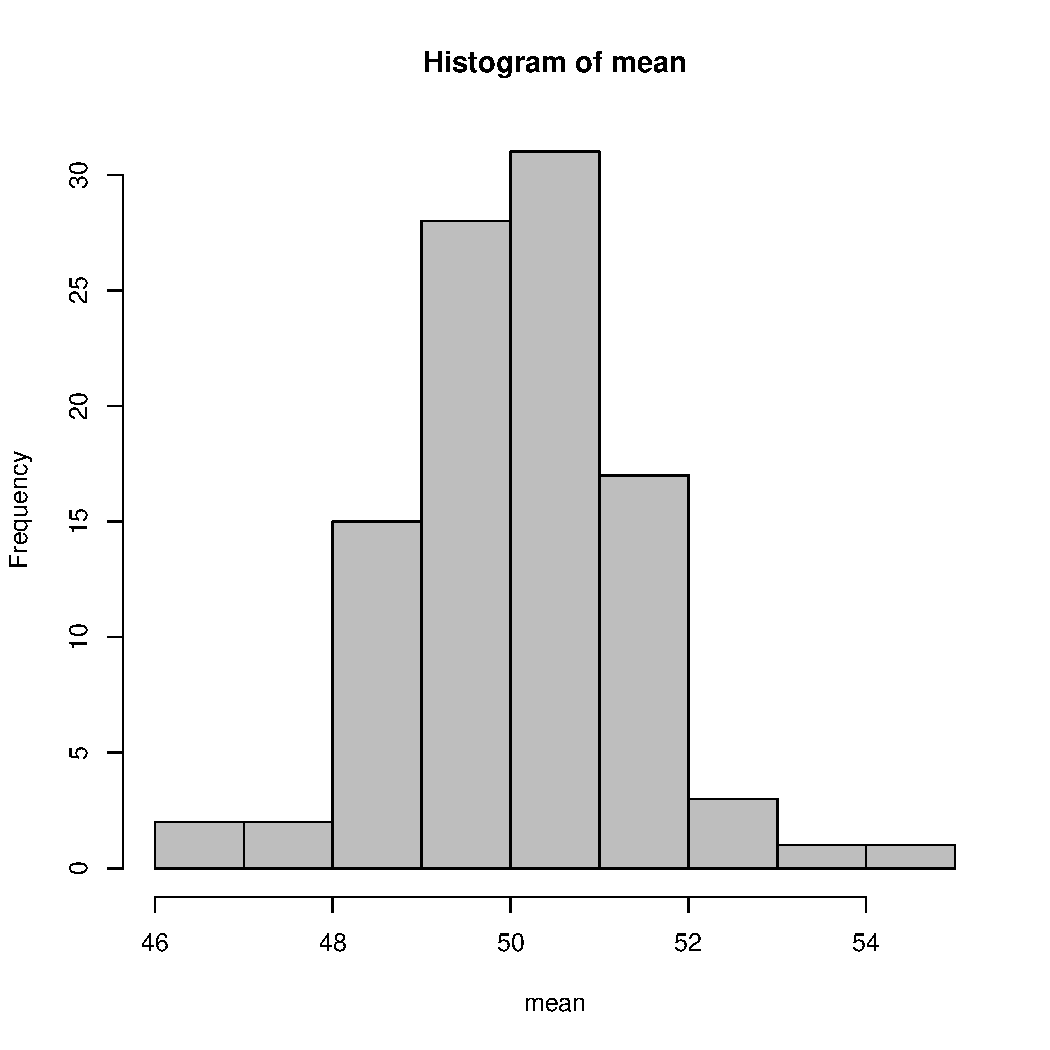
\includegraphics[width=80mm]{pictures/hist_chisq.pdf}
\end{center}
}

\frame{
\frametitle{Problem Set 3.6 (b)}
\begin{itemize}
\item[(b)] (5 marks) Repeat the steps in (a) for each combination of 100 and 1000 $\chi^2$ distributed variables and for each of 50, 100, 1000, 10000 observations. 
Comment on what you observe in each histogram you create with increasing number of observations and increasing number of created random variables.
\end{itemize}
\pause

My hunch: better to do point (c) first, otherwise we have to repeat the code from point (a) 8 different times!
}

\frame{
\frametitle{Problem Set 3.6 (b) -- output}
\begin{figure}
  \centering
  \subfloat{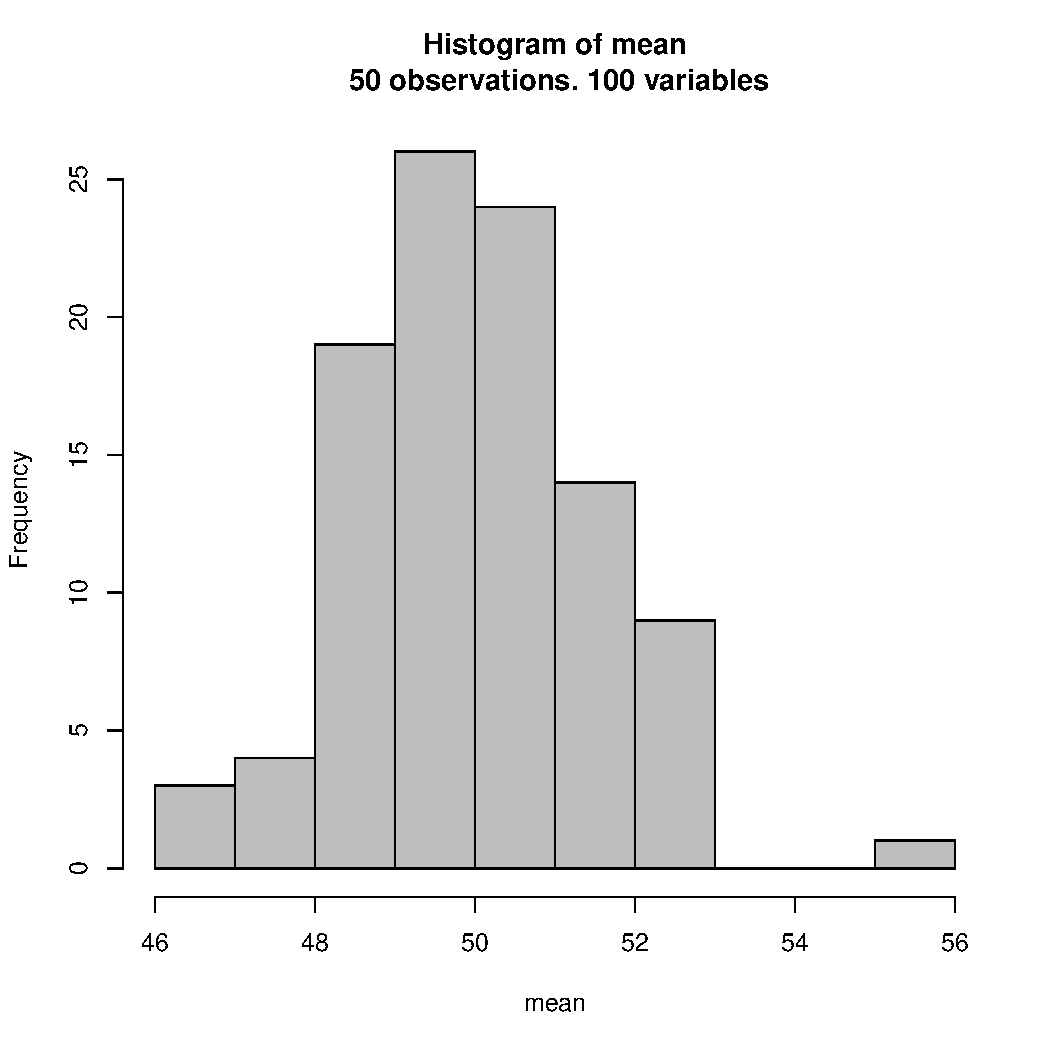
\includegraphics[width=50mm]{pictures/obs50var100.pdf}}\qquad
  \subfloat{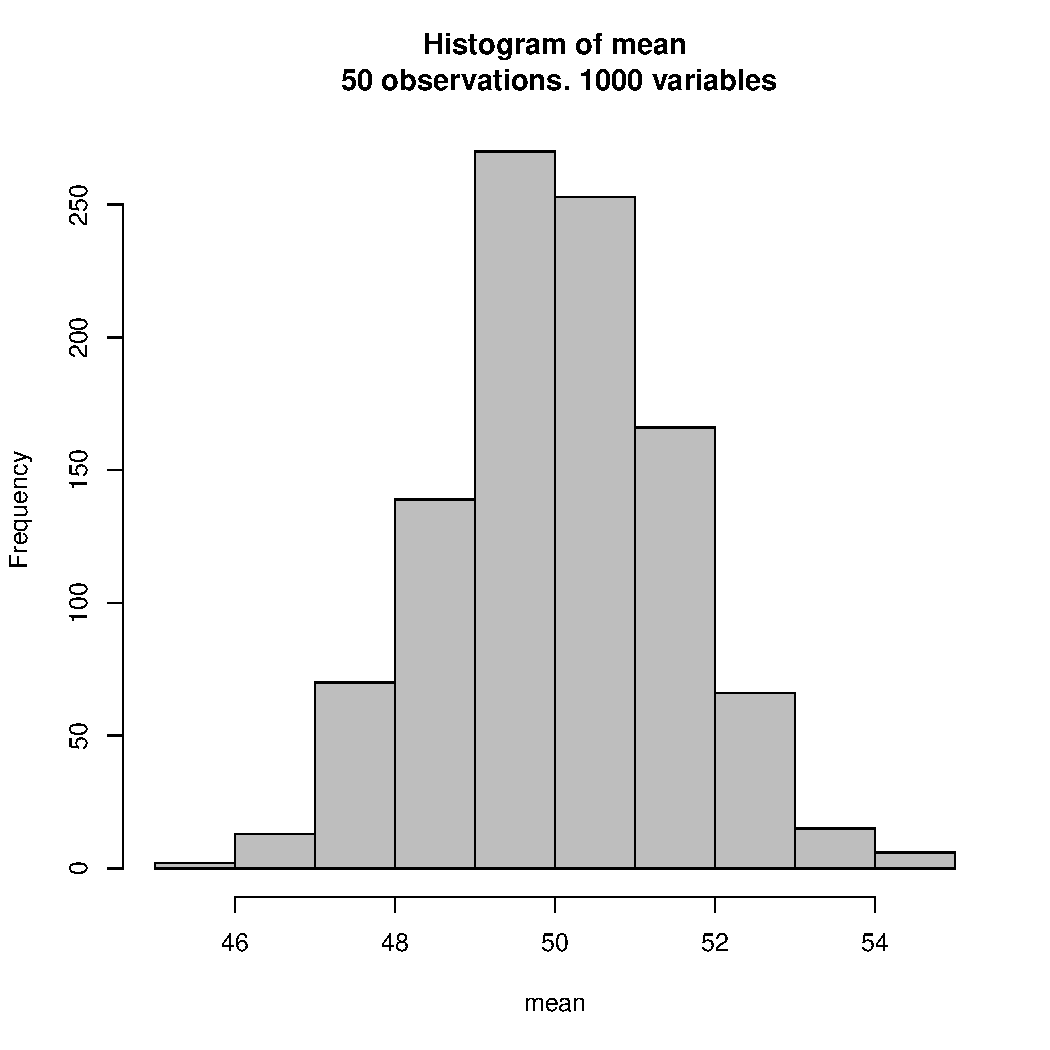
\includegraphics[width=50mm]{pictures/obs50var1000.pdf}}
\label{fig:fig}
\end{figure}
}

\frame{
\frametitle{Problem Set 3.6 (b) -- output}
\begin{figure}
  \centering
  \subfloat{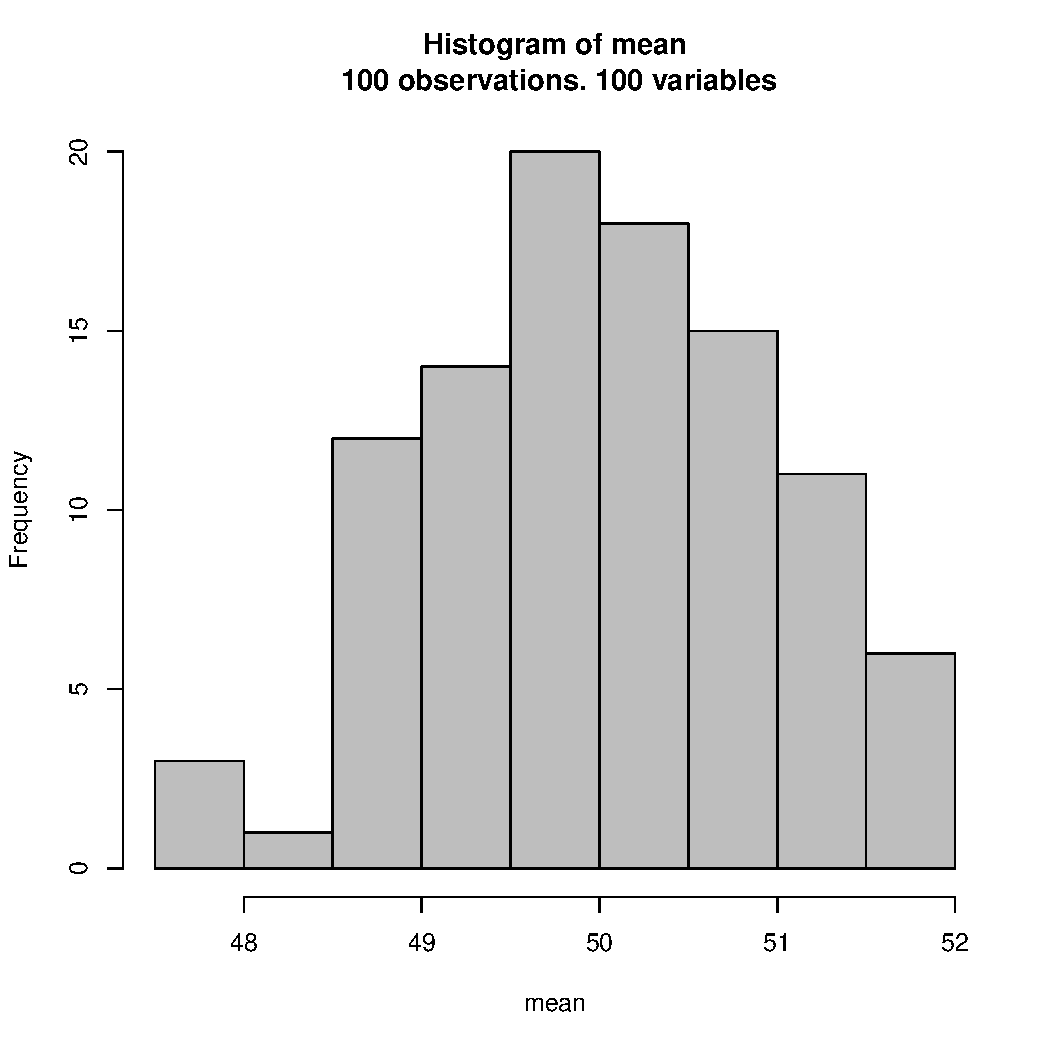
\includegraphics[width=50mm]{pictures/obs100var100.pdf}}\qquad
  \subfloat{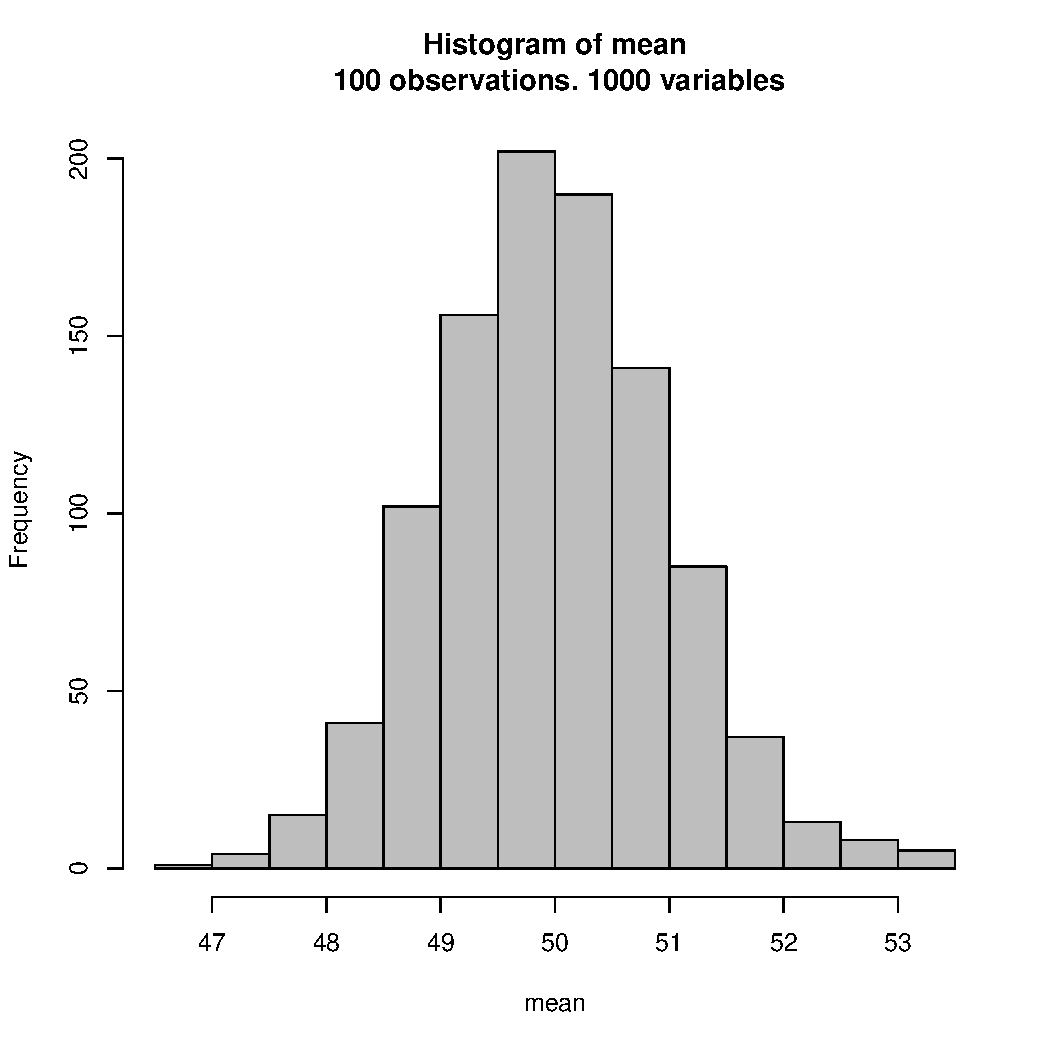
\includegraphics[width=50mm]{pictures/obs100var1000.pdf}}
\label{fig:fig}
\end{figure}
}

\frame{
\frametitle{Problem Set 3.6 (b) -- output}
\begin{figure}
  \centering
  \subfloat{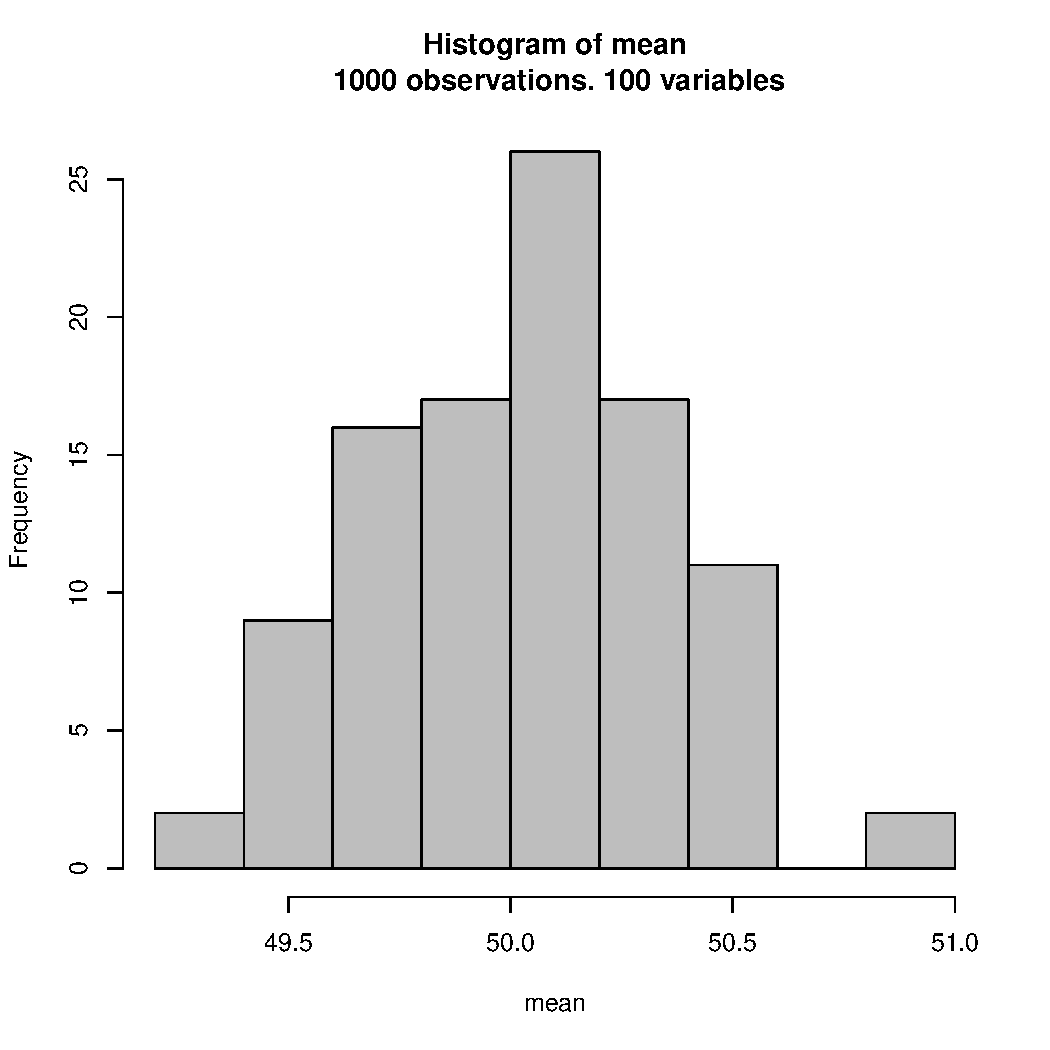
\includegraphics[width=50mm]{pictures/obs1000var100.pdf}}\qquad
  \subfloat{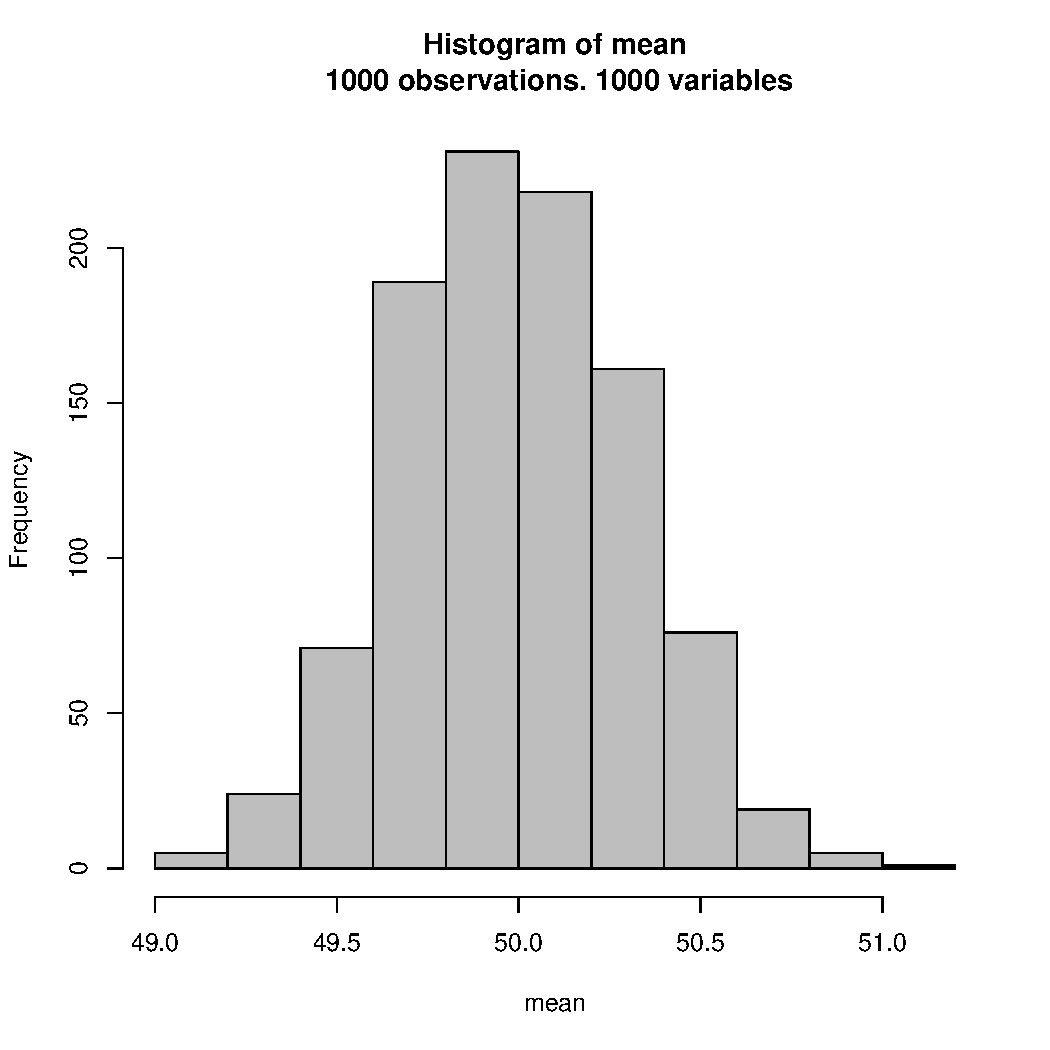
\includegraphics[width=50mm]{pictures/obs1000var1000.pdf}}
\label{fig:fig}
\end{figure}
}

\frame{
\frametitle{Problem Set 3.6 (b) -- output}
\begin{figure}
  \centering
  \subfloat{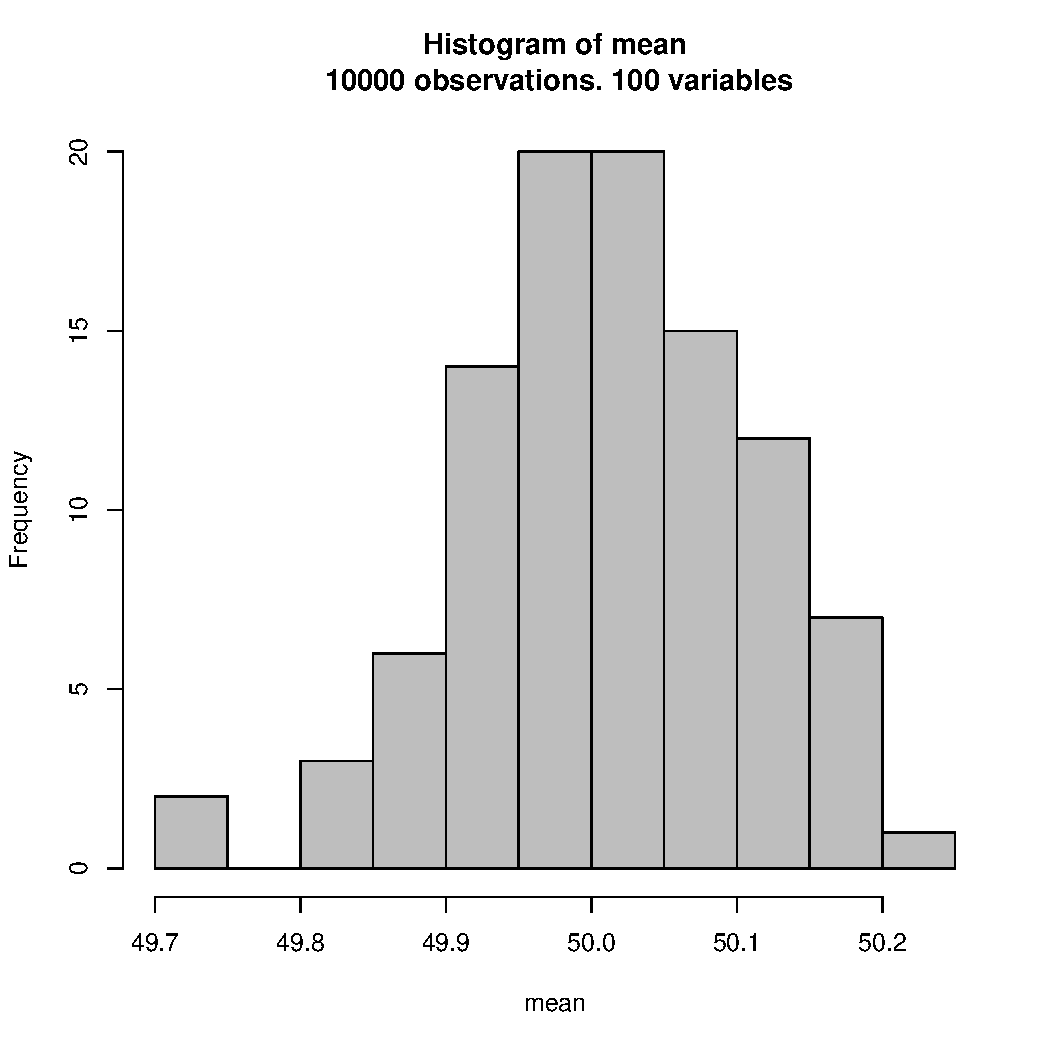
\includegraphics[width=50mm]{pictures/obs10000var100.pdf}}\qquad
  \subfloat{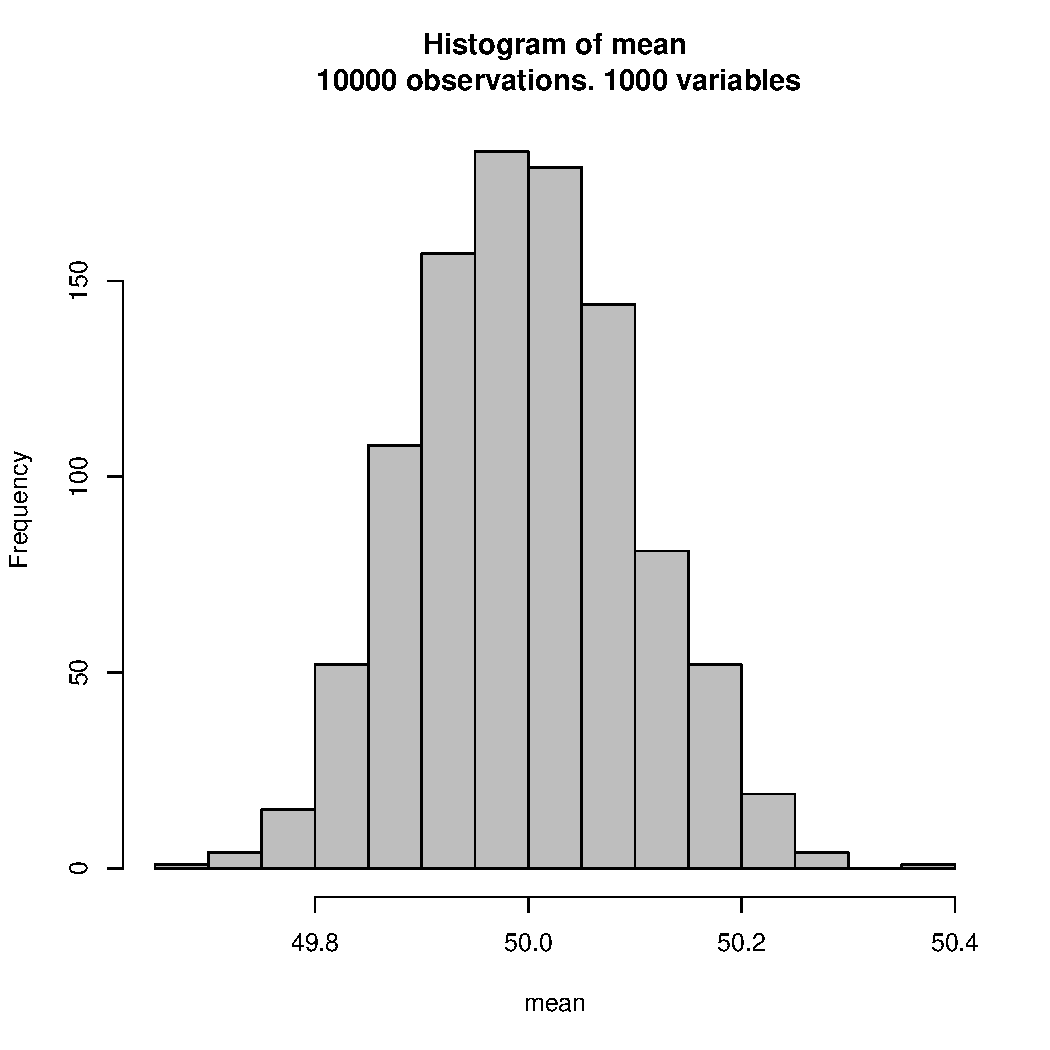
\includegraphics[width=50mm]{pictures/obs10000var1000.pdf}}
\label{fig:fig}
\end{figure}
}

\begin{frame}[fragile]
\frametitle{Problem Set 3.6 (c)}
\begin{itemize}
\item[(c)] (8 marks) Finish the \texttt{Stata program} or \texttt{R function}
\end{itemize} \pause
In R:
\begin{lstlisting}[language = R]
chi2histogram <- function(n,df=50,m){
  mean <- rep(NA, m)
  for (i in 1:m) {
    mean[i] <- mean(rchisq(n, df, ncp = 0))
  }
  hist(mean, col = "gray")
}
\end{lstlisting}
\end{frame}

\begin{frame}[fragile]
\frametitle{Problem Set 3.6 (c)}
\begin{itemize}
\item[(c)] (8 marks) Finish the \texttt{Stata program} or \texttt{R function}
\end{itemize} \pause
In Stata:
\begin{lstlisting}
program drop _all
program chi2histogram
	args m n
    local N = `n'*`m'
    set obs `N'
    g varMean = .
    forvalue i = 1/`m' {
    	tempvar chi2Var
       	g `chi2Var' = rchi2(50)
       	sum `chi2Var'
       	replace varMean = r(mean) in `i'}
	hist varMean, name(hist`m'_`n', replace) title("N=`n', Variables=`m'", col(black)) xsc(off)
end
\end{lstlisting}
\end{frame}

\frame{
\frametitle{Problem Set 3.7}
\begin{enumerate}
\item[7.] (15 marks) Tory backbenchers define a terrible leader as one who loses 7 out of 10 votes. We observed that Johnson got 3 out of 4 bills voted into law. 
We are testing the claim that Boris Johnson is a terrible leader, expressed in binomial distribution parameters, we test
whether the success probability of the event ``lose a vote'' is $p=.7$. If we cannot reject that hypothesis, then Boris Johnson may be called a terrible leader. The PMF under this null hypothesis applied to the observed data of 4 bills brought to the parliament floor is:
\begin{itemize}
\item[] $P(X=0)=.0081$, $P(X=1)=.0756$
\item[] $P(X=2)=.2646$, $P(X=3)=.4116$ 
\item[] $P(X=4)=.2401$
\end{itemize}
\end{enumerate}
}

\frame{
\frametitle{Problem Set 3.7 (a)}
\begin{enumerate}
\item[(a)] (10 marks) Now, say the desired level of statistical significance is $\alpha=.05$. Given that we observe Boris Johnson winning 3 out of 4 bills, are you able to reject the null hypothesis stated above? Provide a p-value associated with this hypothesis test.
\end{enumerate}
\pause
Say the null hypothesis is true, then observing that Boris loses only one vote or less occurs with probability $P(X=1)+P(X=0)=.0756+.0081=.0837$. That's our p-value for this hypothesis test. Under the null-hypothesis there is a probability of $0.0837$ to observe Boris losing only 1 vote out of 4 (which is what we observe). Thus we cannot reject the null hypothesis at $\alpha=.05$.
}

\frame{
\frametitle{Problem Set 3.7 (b)}
\begin{enumerate}
\item[(b)] (3 marks) In this example, what would be the lowest level of significance at which you could reject a null hypothesis?
\end{enumerate} \pause
The lowest level at which you could reject the null hypothesis with this data is $\alpha\leq.01$. We would arrive at a p-value of $.0081$ if we would observe Boris Johnson winning 4 out of 4 votes (losing no vote or $x=0$). Then, we clearly would have to reject the null hypothesis that he is a terrible leader.
}

\frame{
\frametitle{Problem Set 3.7 (c)}
\begin{enumerate}
\item[(c)] (2 marks) Above, you see an \textbf{exact} probability distribution to help you conduct a hypothesis test. Name and explain two more ways how you could generate a test distribution. Give an example of the context in which you have seen one of the two other ways to generate a test distribution.
\end{enumerate}
\pause
PMF of $X$ is obtainable by simulation or theoretical derivation.
\begin{itemize}
\item Simulation: draw a large number of samples of four votes from an underlying binomial distribution with $p=.7$ and $n=4$. 
\item Theoretical derivations: use knowledge of the behaviour of probability distributions (Bernoulli trials and formulas). 
\end{itemize}

Not appropriate here but the PMF of a binomially distributed random variable with more potential realizations and a large number of samples can be approximated by a normal PDF over $X$.
}

\frame{
\frametitle{Conclusion}

\begin{center}
All clear? Questions? \\
Thanks and see you next week!
\end{center}
}

\end{document}